\pagestyle{empty}
\tikzstyle{every picture}+=[remember picture]
\everymath{\displaystyle}
\begin{figure}[!ht]
\centering
\scalebox{.8}{

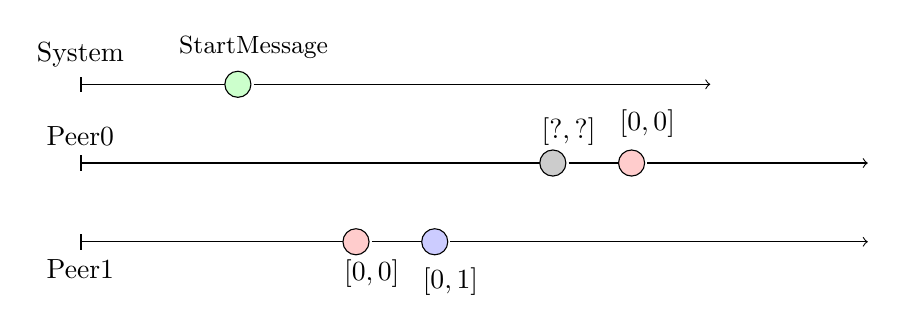
\begin{tikzpicture}

% SYSTEM
\draw[|-] (0,2) node[above=1mm]{System} -- (2,2) node{\tikz[baseline]{
	\node[fill=green!20,draw,circle] (sm){};
}};
\draw[->] (2.2,2) node[above=2mm]{\small{StartMessage}} -- (8,2) {};

% PEER 0
\draw[|-] (0,1) node[above=1mm]{Peer0} -- (6,1) node{\tikz[baseline]{
	\node[fill=black!20,draw,circle] (f0){};
}};
\draw[-] (6.2,1) node[above=1mm]{$[?,?]$} -- (7,1) node{\tikz[baseline]{
	\node[fill=red!20,draw,circle] (f1){};
}};
\draw[->] (7.2,1) node[above=2mm]{$[0,0]$} -- (10,1) node[below=1mm]{};

% PEER 1
\draw[|-] (0,0) node[below=1mm]{Peer1} -- (3.5,0) node{\tikz[baseline]{
	\node[fill=red!20,draw,circle] (e0){};
}};
\draw[-] (3.7,0) node[below=1mm]{$[0,0]$} -- (4.5,0) node{\tikz[baseline]{
	\node[fill=blue!20,draw,circle] (e1){};
}};
\draw[->] (4.7,0) node[below=2mm]{$[0,1]$} -- (10,0) node[below=1mm]{};

\end{tikzpicture}

\begin{tikzpicture}[overlay]
  \path[->] (sm) edge [out=-90, in=135] (e0);
  \path[->] (sm) edge [out=-45, in=135] (f1);
  \path[->] (e1) edge [out=45, in=-135] (f0);
\end{tikzpicture}

}

  \caption{An overcomed issue in our asyncronous simulation.}
\end{figure}
